\documentclass{article}
% \usepackage{biblatex}
\usepackage{amsmath}
\usepackage{graphicx} % Required for inserting images
\usepackage{hyperref}
\usepackage{amsfonts}
\usepackage{amssymb}
\usepackage{amsthm}

\newtheorem{theorem}{Theorem}

\begin{document}
\title{RECAP Capstone Project: \\ The Attention Neuron Is Not \\ Truly Permutation Invariant}
\author{Chuen Yang Beh}
\date{June 2025}

\maketitle

\begin{abstract}
The Attention Neuron \cite{Tang-and-Ha-2021} is a peculiar RL policy architecture which claims
to create permutation-invariant representations of an agent's observations. In this week-long project, we observe that the architecture \textbf{can} conceptually be permutation invariant,
but prove empirically that the implementation by Tang and Ha \cite{Tang-and-Ha-2021}
is \textbf{not} permutation invariant in practice, due to the use of recurrent LSTM states
in a permutation-sensitive manner. Fascinatingly, however, we observe that the architecture is \textbf{nonetheless resilient} to permutations of the observation vector.
As such, we investigate how this architecture achieves this astonishing property through 
visualizations, ablations, and mathematical analysis on a toy environment (CartPoleSwingUpHarder \cite{Freeman-et-al-2019}).
\end{abstract}

% Directions before tmr
% 1. When you perturb observations, also zero the hidden states.
%   Purpose: Check if model is starting from a clean slate when it gets perturbed.
% 2. When you perturb observations, also perturb the hidden states. ("Cheat" setup)
%   Check if the bad performance is simply due to the hidden states not actually being invariant.
% 3. (Write as a future direction) How many GD steps does it take to make the model more robust? (vs, say, an MLP model)

\section{Introduction}

The Attention Neuron architecture \cite{Tang-and-Ha-2021} appears to be motivated
from a neuroscience perspective. The authors observe that humans are sometimes capable
of orienting themselves despite "sensory substitutions" (e.g. riding a bike backwards instead of forwards).
Justifying that this would imbue robustness and generalisability in agents' capabilities,
the authors then propose the Attention Neuron architecture as a way to achieve this property.

While the authors' results \cite{Tang-and-Ha-2021} are extremely promising and reproducible, our experiments reveal 
that the implementation of the Attention Neuron architecture
is not truly permutation invariant, due to the use of recurrent LSTM states 
in a permutation-sensitive manner.

\section{Preliminary: The Attention Neuron}

Drawing inspiration from the Set Transformer architecture \cite{Lee-et-al-2019}, the Attention Neuron 
architecture claims to achieve permutation invariance by using cross-attention,
where the query vector is a set of learned positional embeddings, the key vector consists of observation 
and previous-action features, and the value vector is the observation vector itself.

\subsection{Architecture Overview}
A figure of the architecture is shown in Figure \ref{fig:attention_neuron_architecture}.
\begin{figure}[h]
    \centering
    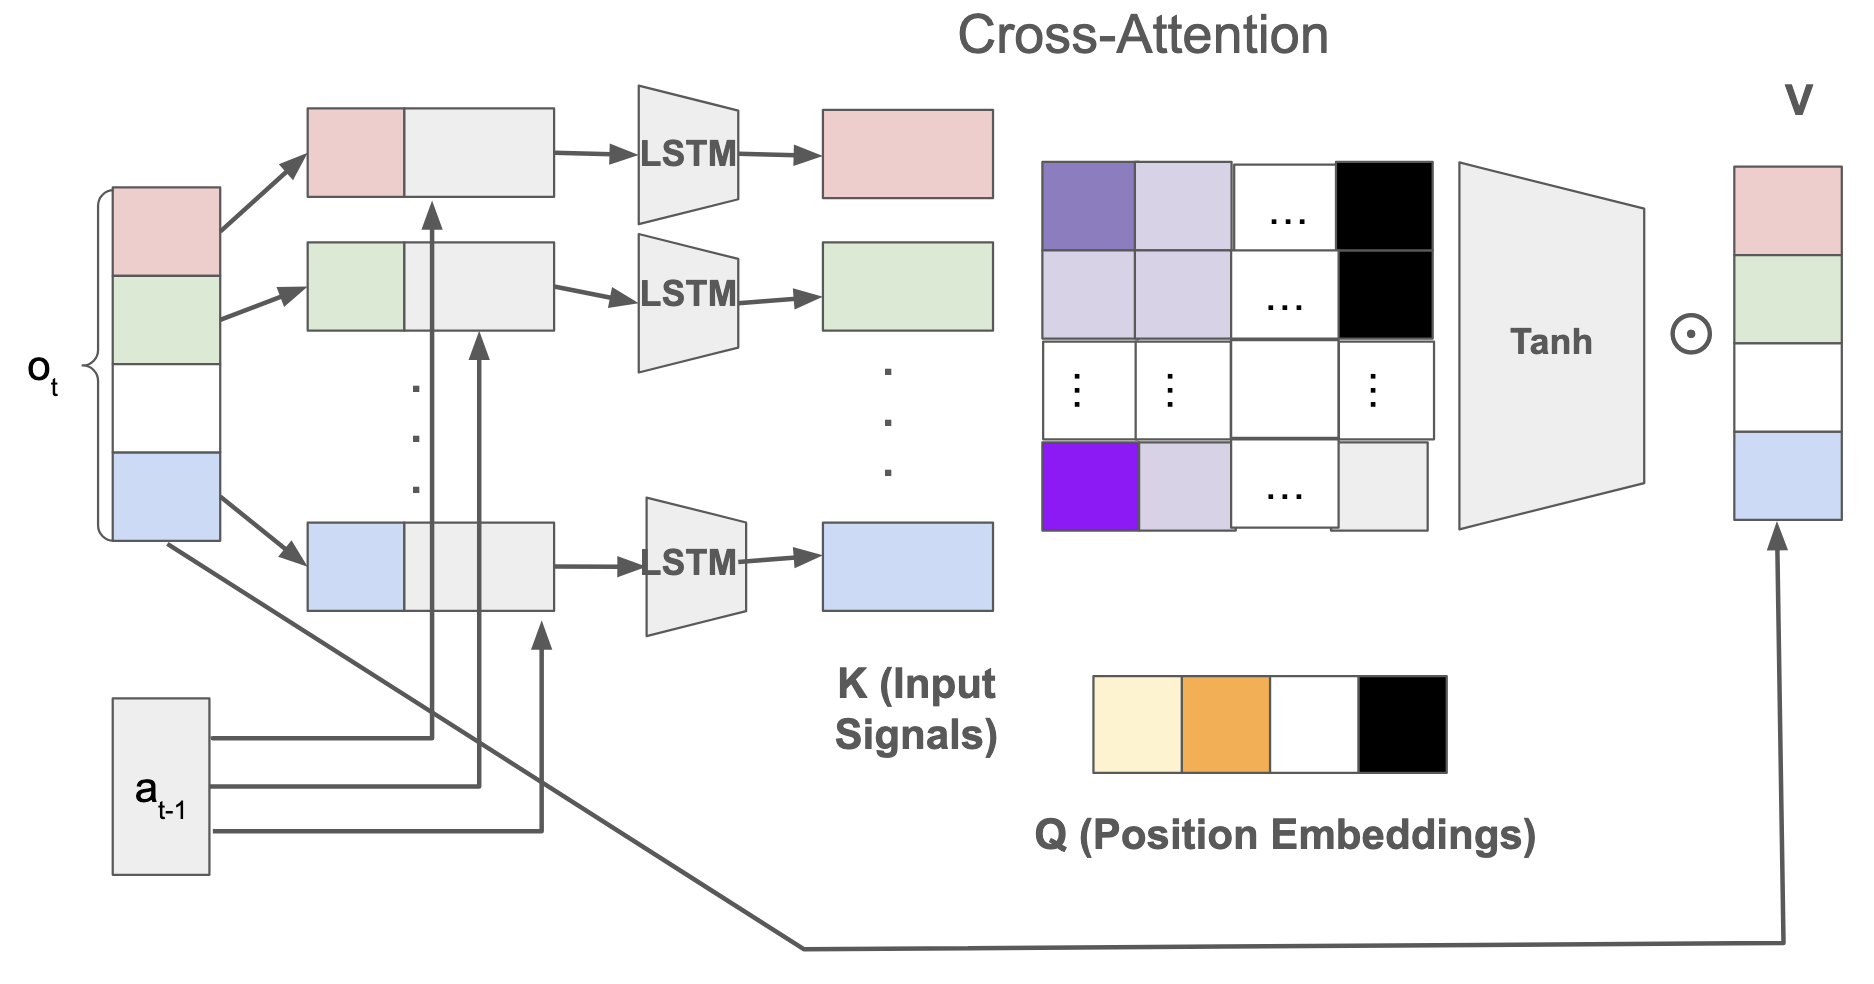
\includegraphics[width=0.8\textwidth]{images/attention_neuron.png}
    \caption{The Attention Neuron architecture from \cite{Tang-and-Ha-2021}, redrawn for clarity.}
    \label{fig:attention_neuron_architecture}
\end{figure}

At a high level, the architecture's forward pass can be described as follows (at each timestep $t$):
\begin{itemize}
    \item The observation vector $o_t$ at time $t$ is broken up into 
    $d_{obs}$ \textit{signals}, $\{o_{t,1}, o_{t,2}, \ldots, o_{t,d_{obs}}\}$.
    \item The signals are then independently concatenated with the previous action $a_{t-1}$,
    forming the \textit{info signals} $I_{t,k} = (o_{t,k}) \oplus a_{t-1}$ with dimension $1 + d_{act}$ for $k = 1, 2, \ldots, d_{obs}$.
    \item The info signals (along with hidden LSTM state $h_{t-1}$ and cell state $c_{t-1}$) are then passed (independently) through an LSTM Cell $L$,
        which computes new hidden states $h_t$ of dimension $d_{out}$ and cell states $c_t$ of dimension $d_{out}$.
    \item The LSTM outputs and positional embeddings $P$ are then mixed via bidirectional cross-attention,
        with the query vectors being the positional embeddings $P$ of dim $d_{out}$,
        and the key vectors being the LSTM hidden state $h_t$. 
        \footnote{
            The non-linearity of the attention matrix, rather than being softmax,
            is a $\tanh$ function.
        }
        This results in an attention matrix $A_t$ of dimension $d_{out} \times d_{obs}$.
    \item Finally, the attention matrix $A_t$ is multiplied with the observation vector $o_t$,
        resulting in a feature vector $f_t$ of dimension $d_{out}$. This feature vector
        represents the "digested" observation vector, and is supposed to remain invariant
        to permutations of the observation vector.
\end{itemize}

Mathematically speaking, the forward pass can be written as:
\begin{align*}
    f_t(o_t, a_{t-1}) = \tanh\left(\underbrace{\tanh\left(P\left(\bigoplus_{i=1}^{d_{obs}} L(I_{t,i}, h_{t-1}, c_{t-1})\right)^T\right)}_{A_t} o_t\right)
\end{align*}

where $\oplus$ denotes the concatenation operation (dimension implied), 
$L$ is the LSTM function mapping, and $A_t$ is the attention matrix.

\subsection{Claimed Permutation Invariance of Attention Neuron}
Some manual work and elementary linear algebra intuition shows that the claimed
permutation invariance of the Attention Neuron architecture arises from the fact that
whenever the observation $o_t$ is permuted along its rows, the column space of $A_t$ would theoretically
be permuted the same way. Hence $A_t' o_t' = A_t o_t$.

This forms a basis for the authors' claim that the Attention Neuron architecture is permutation invariant
\cite{Tang-and-Ha-2021}.

Unfortunately, the authors do not provide a formal proof of this claim,
and the decision to use an LSTM to model time dependencies
in each info signal $I_{t,k}$ in fact renders the architecture 
\textbf{permutation sensitive}. We prove this empirically in the next section.

% \subsection{Proof of Permutation Invariance}

% One of the interesting properties of the Attention Neuron architecture is its 
% \textbf{THEORETICAL} permutation invariance.

% \begin{theorem}
%     Permutation Invariance: For any $\sigma: \mathbb{Z}_{\leq d_{obs}} \to \mathbb{Z}_{\leq d_{obs}}$,

%     $$P_{\sigma} h_{t-1} = h_{t-1} \land P_{\sigma} c_{t-1} = c_{t-1} \implies f(P_\sigma o_t, a_{t-1}) = f(o_t, a_{t-1})$$

%     where $P_\sigma$ is the permutation matrix corresponding to $\sigma$.
% \end{theorem}
% \begin{proof}
%     Suppose $P_{\sigma} h_{t-1} = h_{t-1}$ and $P_{\sigma} c_{t-1} = c_{t-1}$.
%     Then, under $P_{\sigma}$,
%     $$P_{\sigma} L(o_t, h_{t-1}, c_{t-1}) = L(o_t, h_{t-1}, c_{t-1})$$.
% \end{proof}

\section{Experiments}

\subsection{Choice of Environment}
We tested the Attention Neuron architecture on the CartPoleSwingUpHarder environment \cite{Freeman-et-al-2019}.
It is best thought of as an extremely difficult version of the CartPole environment \cite{Towers-et-al-2024, Sutton-and-Barto-1998},
as the cart not only needs to swing the pole up from a downwards-facing position, but also needs to balance the pole upright
for an extended period of time.

This environment was primarily chosen since it was the simplest of all the environments used
by the authors of the Attention Neuron paper \cite{Tang-and-Ha-2021}. With a low-dimensional observation space
and no hidden layers in the policy architecture, it will be easier to visualize, compare, and contrast the effects of permutations
on the Attention Neuron architecture.

\subsection{Permutations Within Episodes}
Considering that the authors tout the Attention Neuron architecture's robustness to permutations
even within episodes \cite{Tang-and-Ha-2021},
we decided it would be interesting to reproduce the authors' experiments 
in permuting the observation vector $o_t$ multiple times within an episode.

\subsection{Ablations}
We performed the following ablations on the Attention Neuron architecture:
\begin{itemize}
    \item \textbf{Zeroing the LSTM Recurrent State}: We zeroed the LSTM recurrent state at every time step.
    \item \textbf{Resetting the LSTM Recurrent State Every Permutation}: 
        We reset the LSTM recurrent state to zero at whenever the observation vector was permuted.
    \item \textbf{Permuting the LSTM Recurrent State Every Permutation}: 
        We permuted the LSTM recurrent state whenever the observation vector was permuted.        
\end{itemize}

\section{Results \& Discussion}

\subsection{Zeroing the LSTM Recurrent State Causes Model Collapse}
As shown in Figure \ref{fig:attention_neuron_zeroed_lstm},
zeroing the LSTM recurrent state at every time step causes the agent's performance to collapse.

\begin{figure}[h]
    \centering
    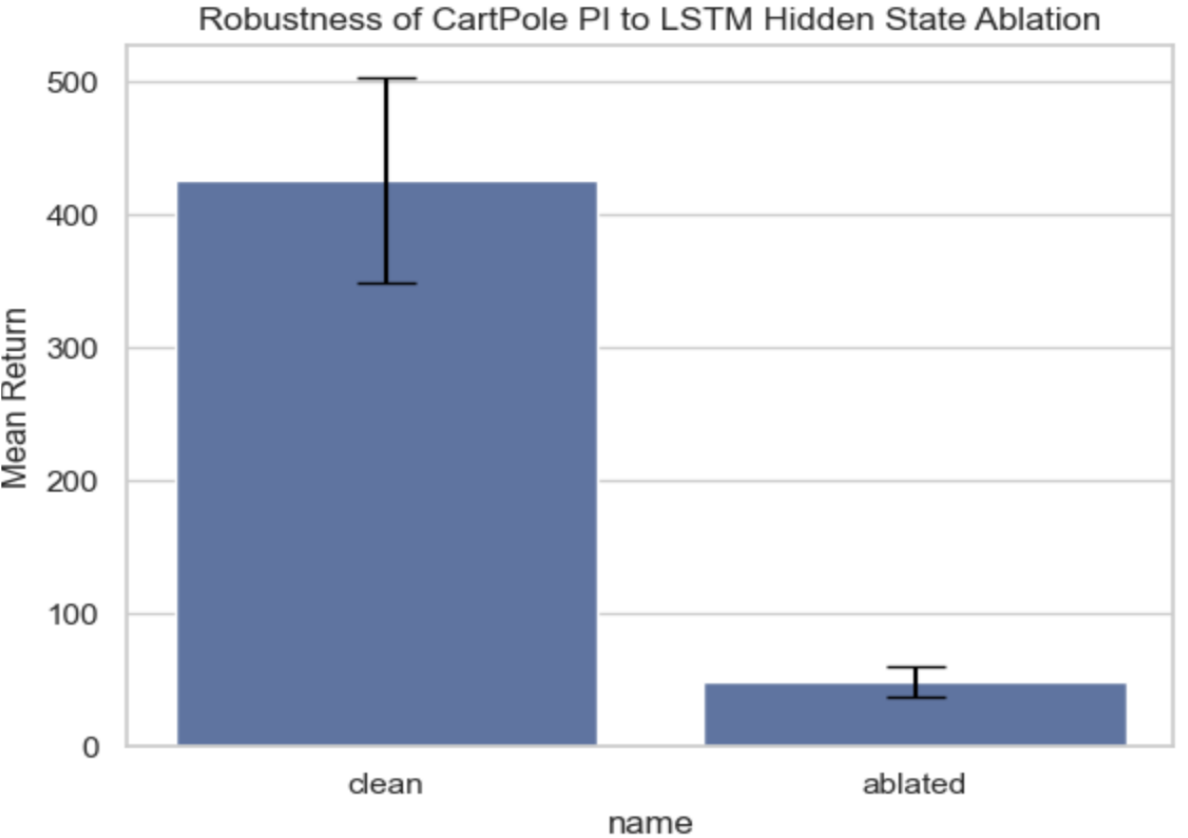
\includegraphics[width=\textwidth]{images/perf_collapse.png}
    \label{fig:attention_neuron_zeroed_lstm}
\end{figure}

While it can be tempting to explain this as the LSTM's pivotal role in the model's success
in CartPoleSwingUpHarder, we note that similar problems have been solved before
using non-recurrent architectures such as MLPs (\cite{ppo-cpsw-2022}).
Hence, it is likely that the policy was simply trained to rely heavily
on the LSTM recurrent state to solve the task.

\subsection{The Attention Neuron Is Robust Against Within-Episode Permutations}

Just as the authors show in their paper \cite{Tang-and-Ha-2021},
we find that the Attention Neuron architecture is robust to permutations of the observation vector
even within an episode.
Figure \ref{fig:attention_neuron_permutation_invariance_within_episode} shows the results of our experiments,
where we permuted the observation vector at every time step within an episode.

\begin{figure}[h]
    \centering
    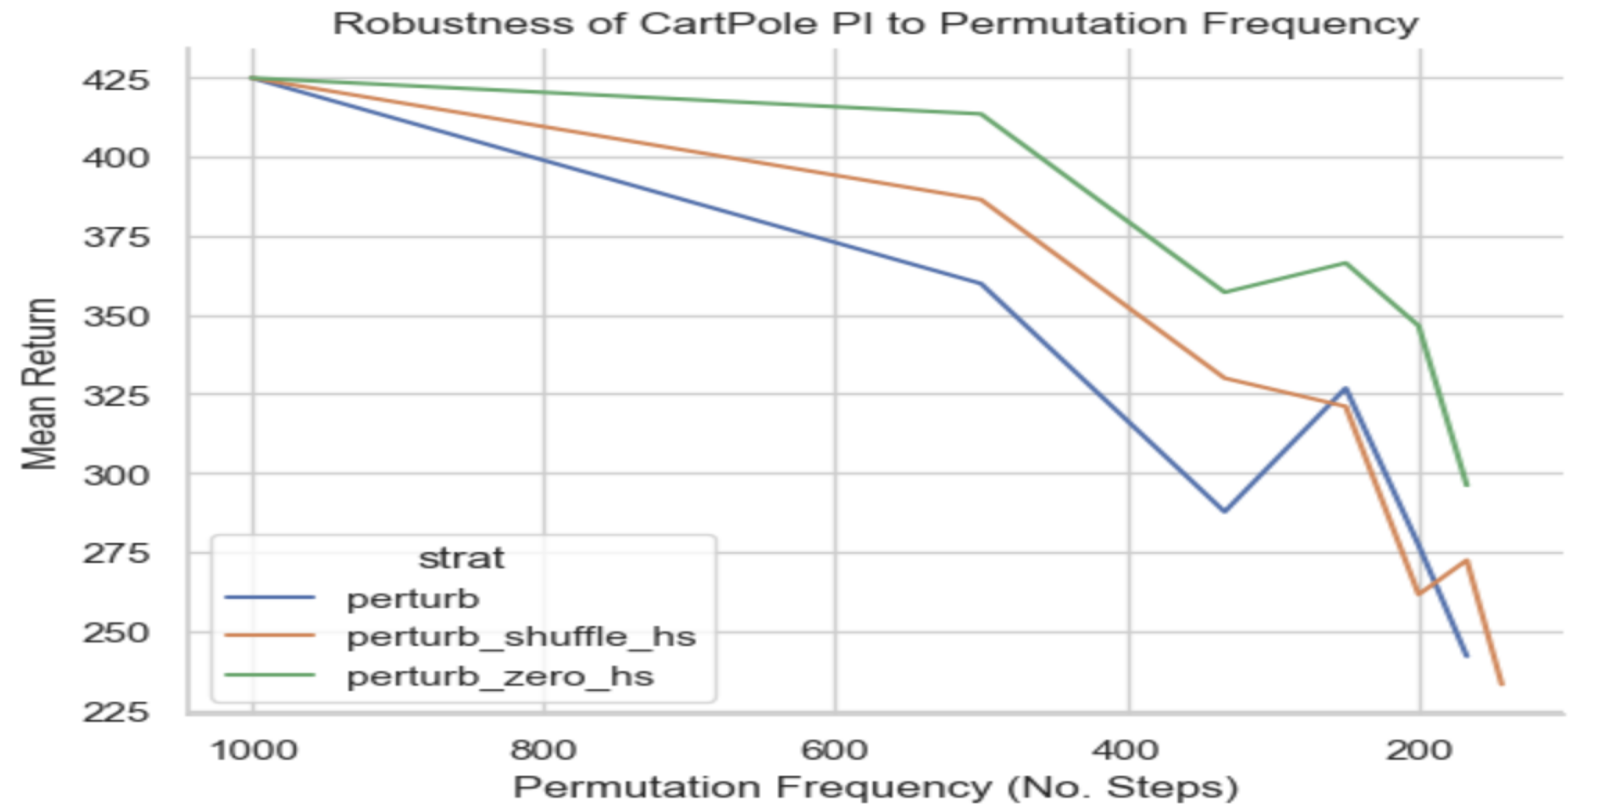
\includegraphics[width=\textwidth]{images/permutation_frequency.png}
    \caption{The Attention Neuron architecture is robust to permutations of the observation vector within an episode.
    }
    \label{fig:attention_neuron_permutation_invariance_within_episode}
\end{figure}

While the performance degrades somewhat, the agent's performance never truly collapses 
like in the previous section,
as would be expected on the usual MLP architecture.
In fact, it is possible to salvage the agent's performance somewhat
through hidden state manipulation, as shown in Figure \ref{fig:attention_neuron_permutation_invariance_within_episode}.

Unfortunately, permuting the LSTM recurrent state in the same way as the observation vector
does not cause the agent's performance to fully recover.
This leads us to believe that the Attention Neuron architecture
may not be truly permutation invariant, for otherwise
the recurrent state permutation would have been sufficient to recover the agent's performance FULLY.

\newpage

\subsection{The Attention Neuron is Not Truly Permutation Invariant}
As shown in Figure \ref{fig:attention_neuron_permutation_invariance},
which is derived from randomly generated rollouts in CartPoleSwingUpHarder,
the Attention Neuron architecture is indeed not truly permutation invariant,
with one notable exception.

\begin{figure}[h!]
    \centering
    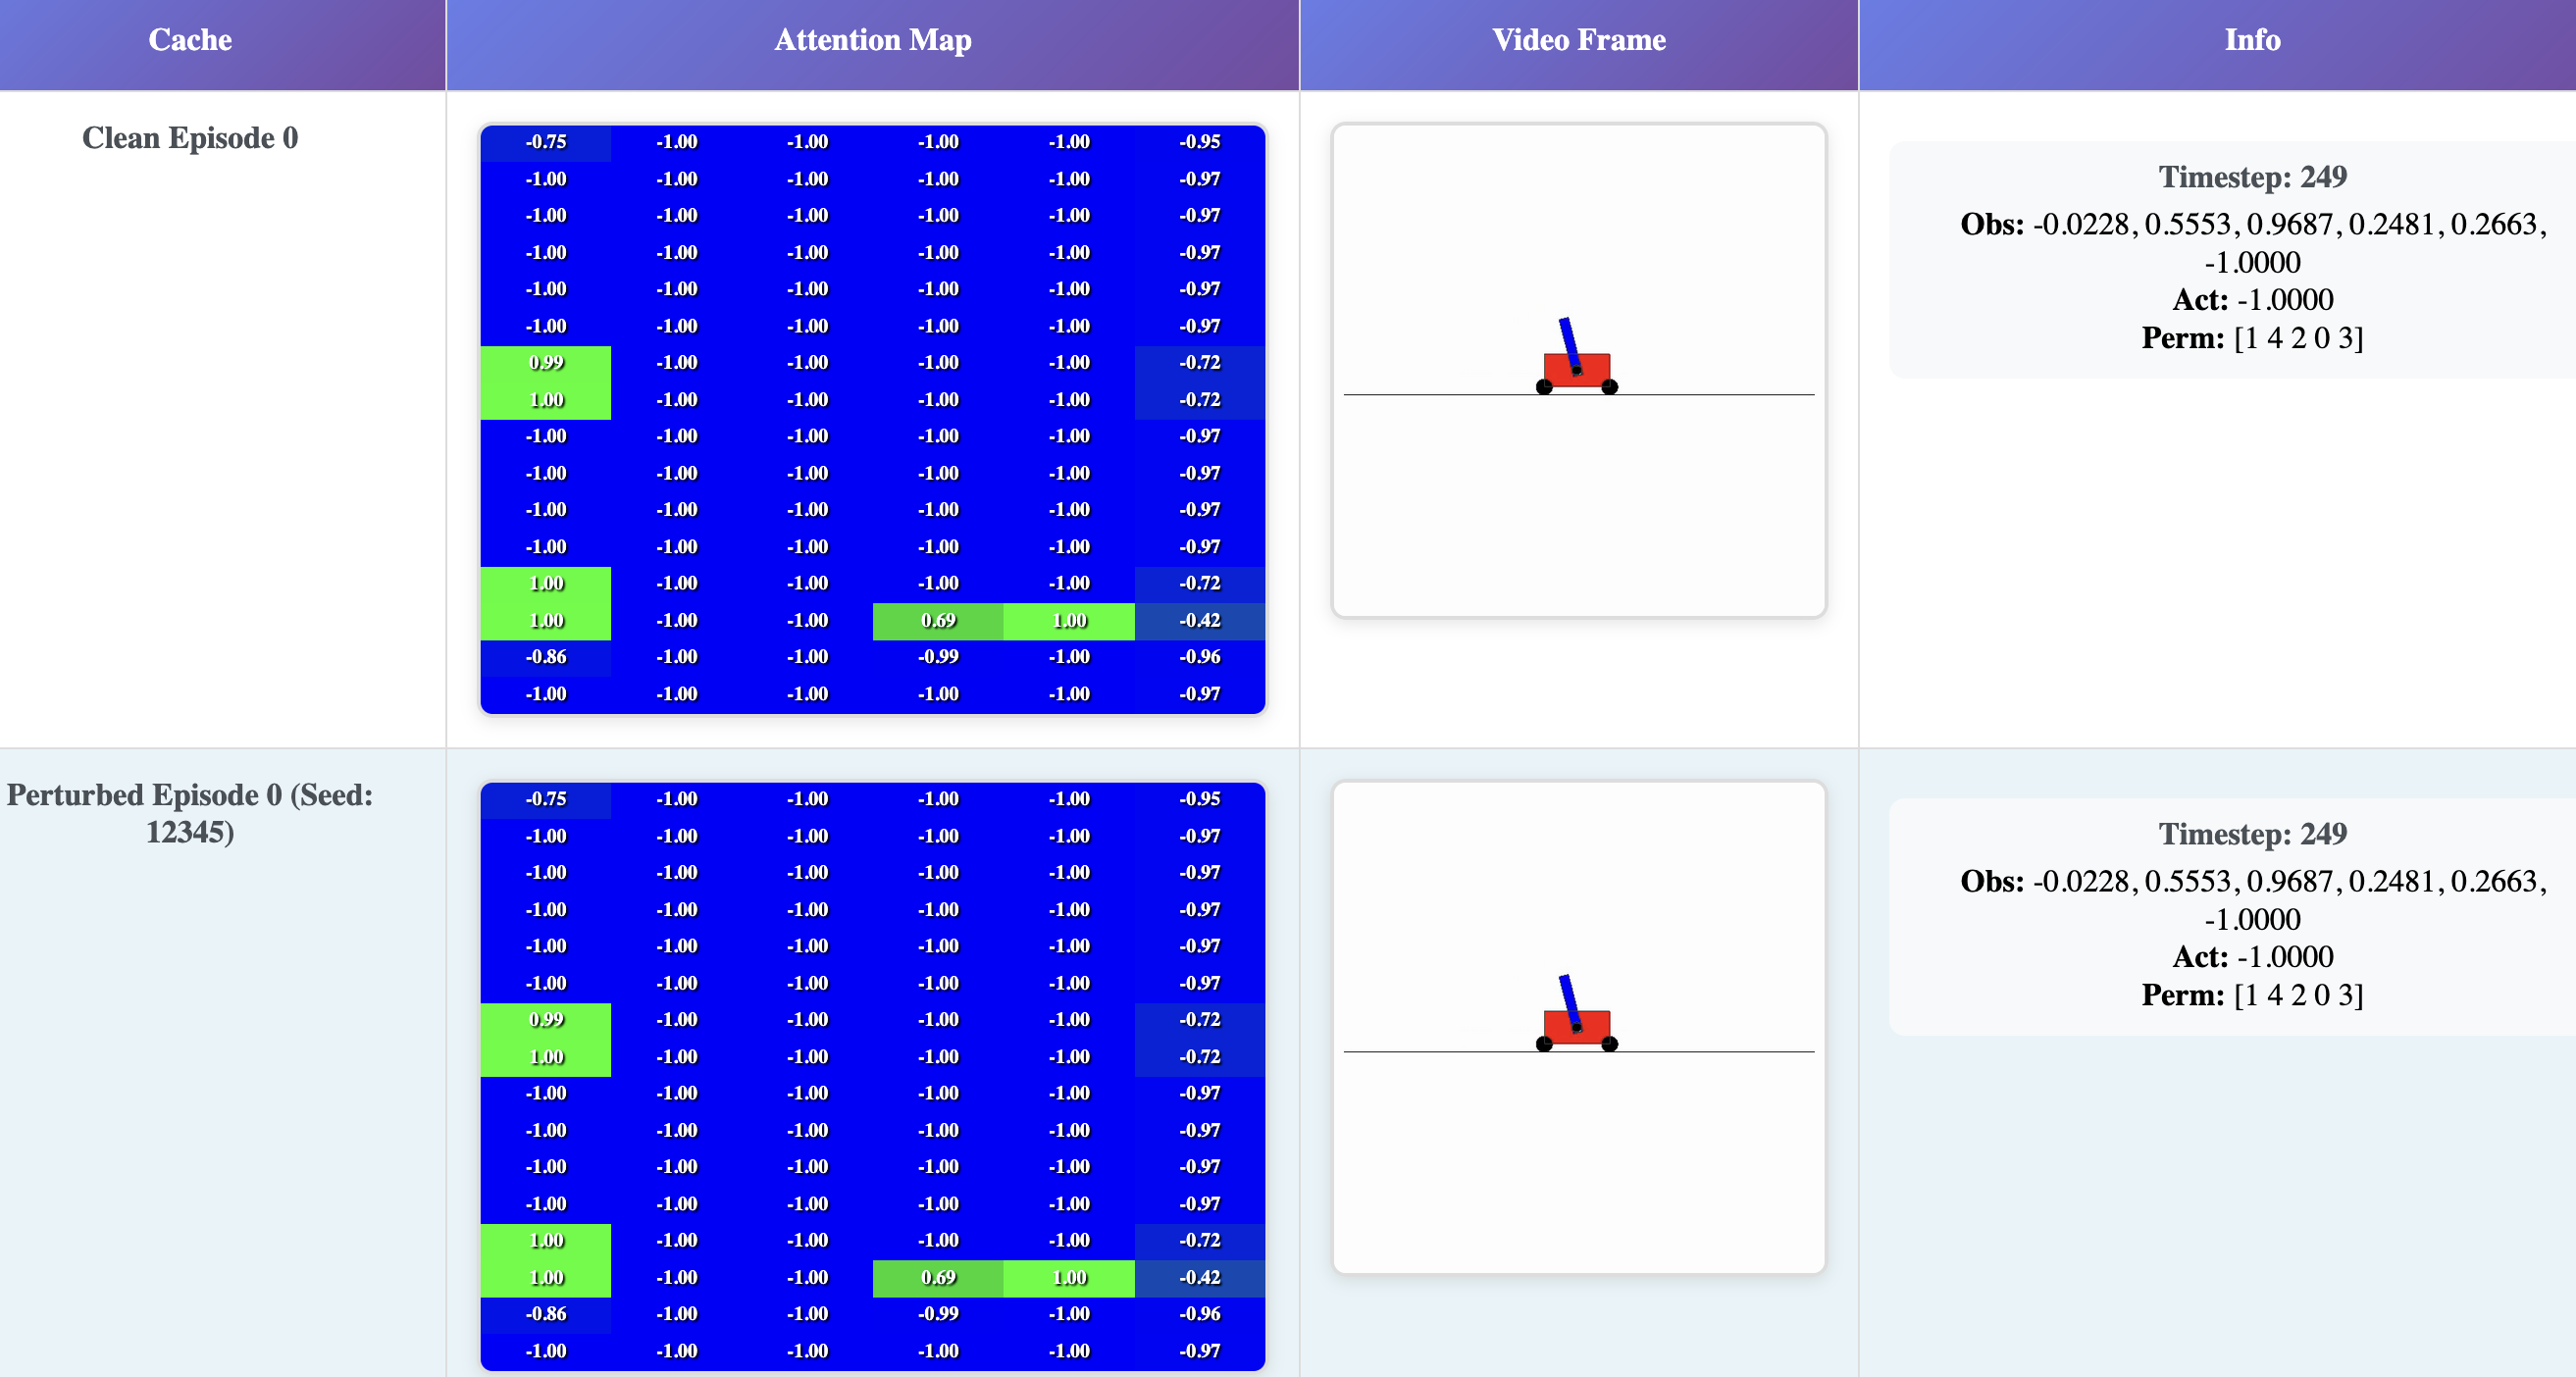
\includegraphics[width=\textwidth]{images/was_identical.png}
    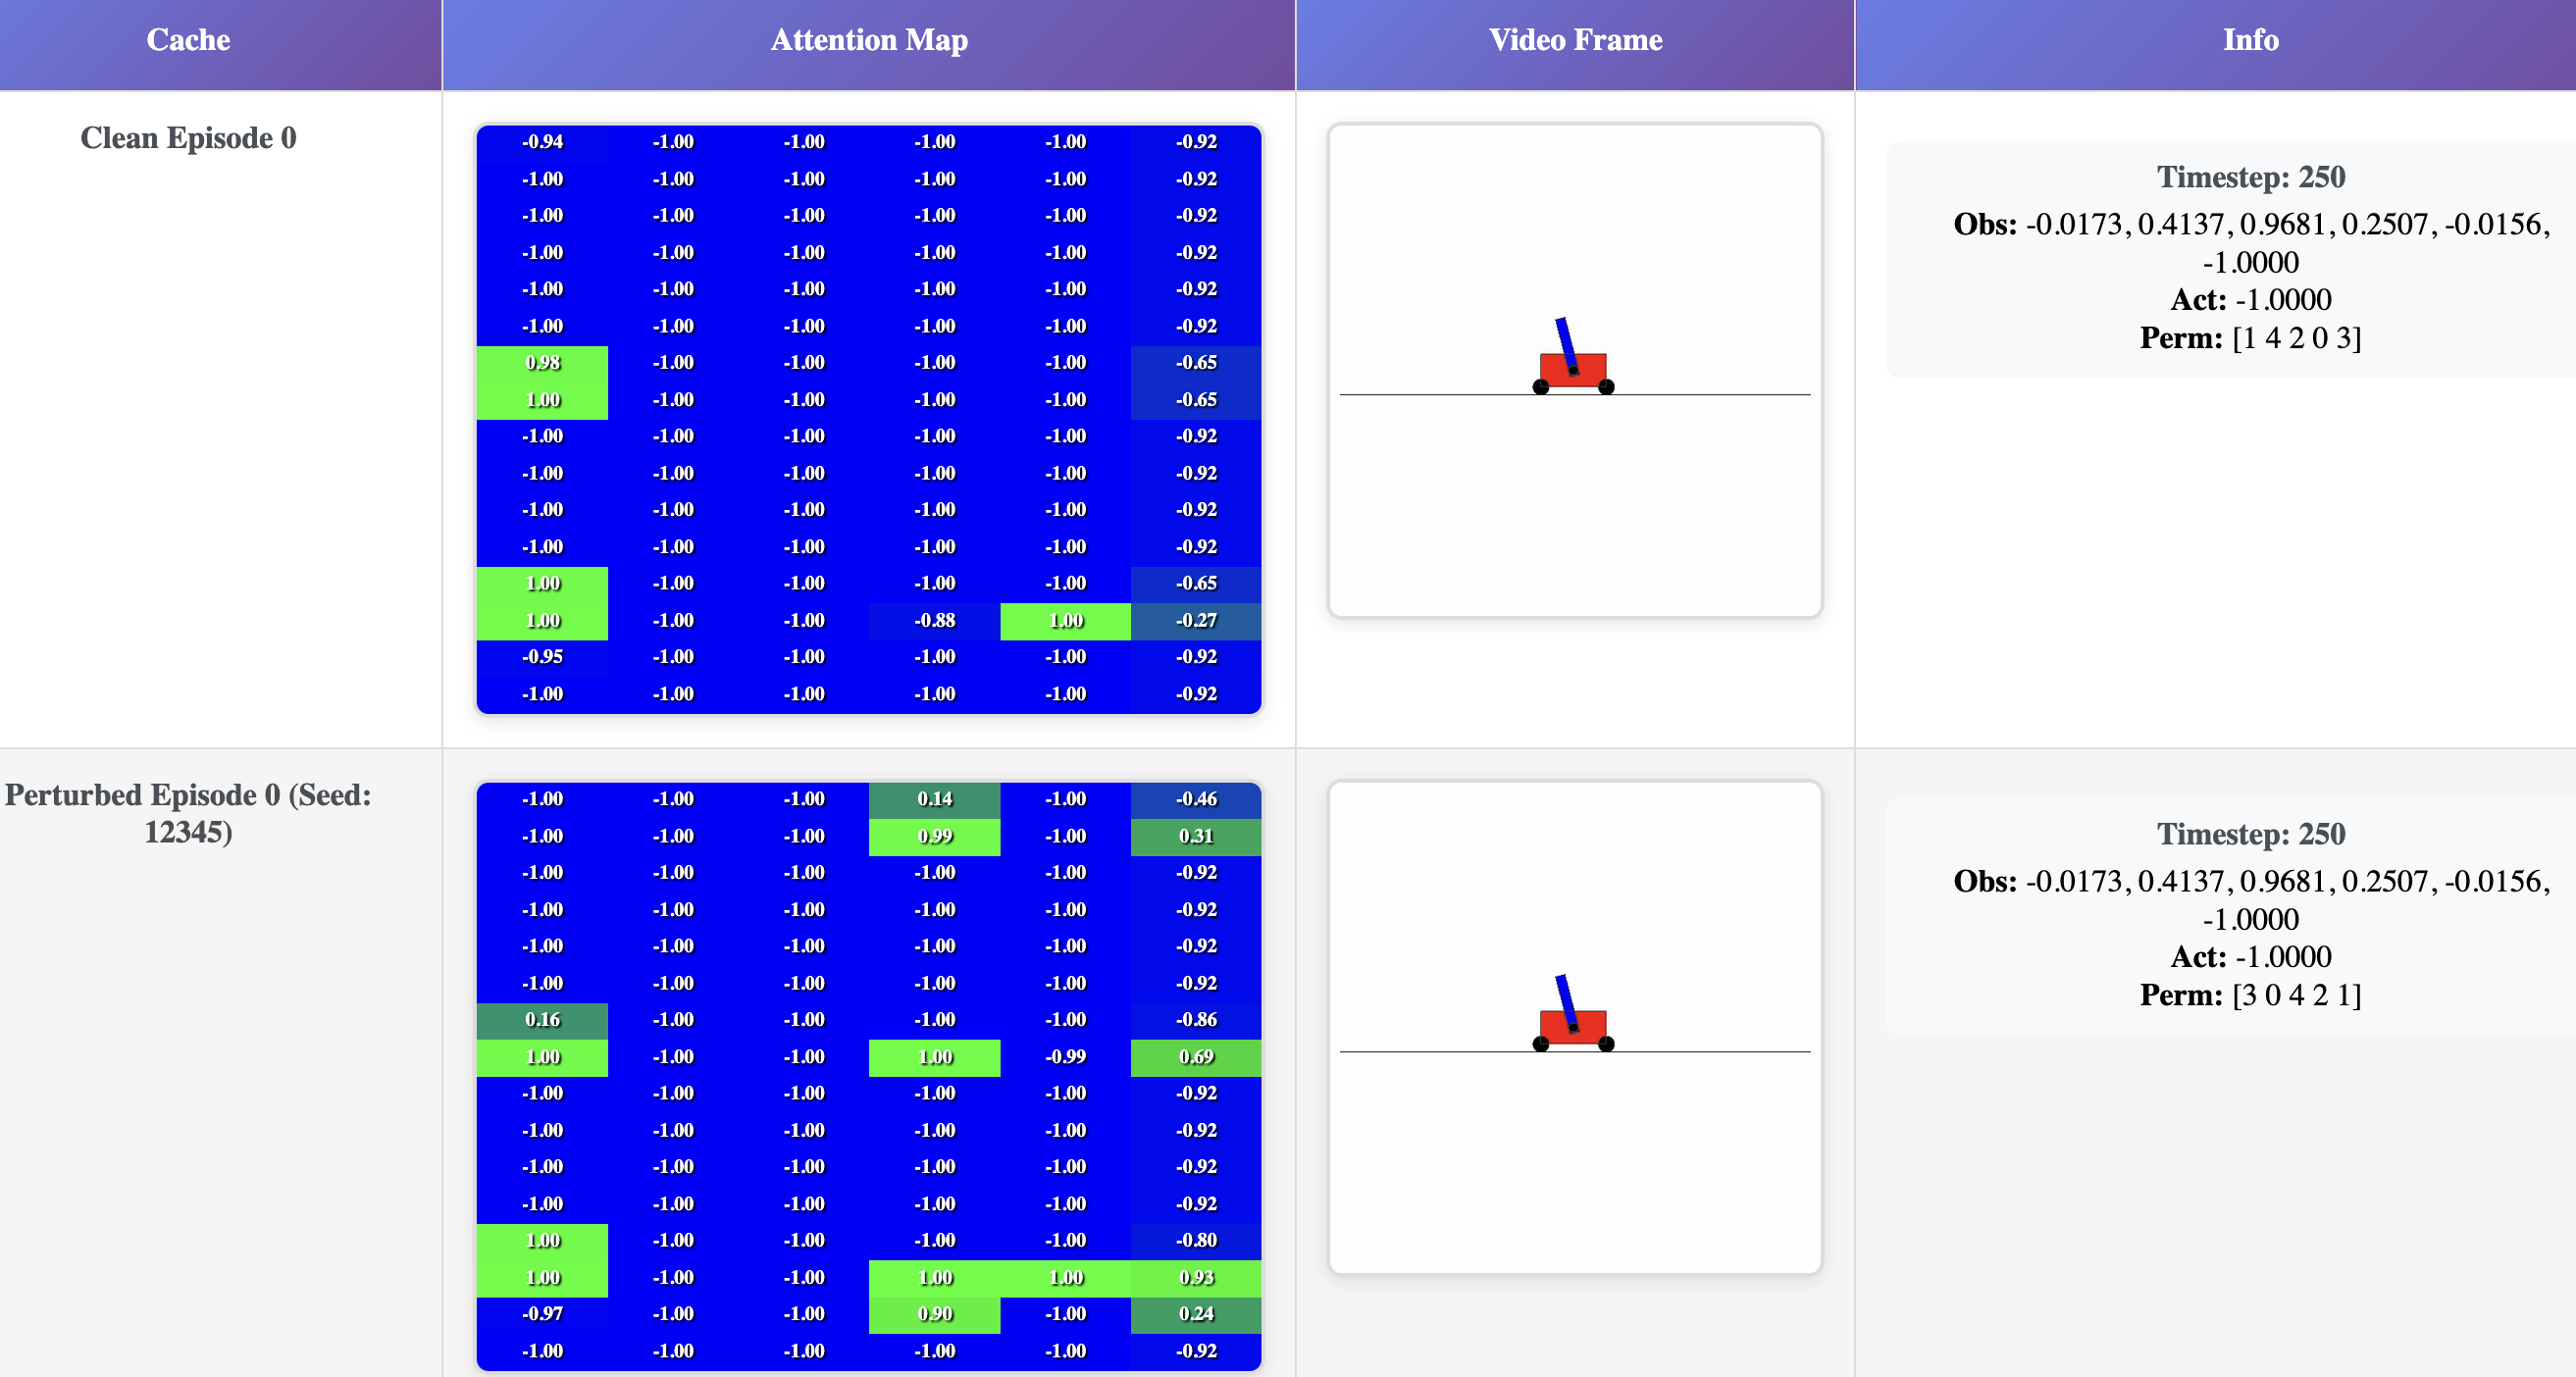
\includegraphics[width=\textwidth]{images/not_permutation_invariant.png}
    \caption{Notice how the attention masks (below) are no longer identical even after accounting for the permutation of the observation vector (above). This shows that the Attention Neuron architecture is not truly permutation invariant, as the LSTM recurrent state is not invariant to permutations.}
    \label{fig:attention_neuron_permutation_invariance}
\end{figure}

If we ablate the LSTM recurrent state by zeroing it at every time step,
the Attention Neuron architecture becomes permutation invariant, as shown in Figure \ref{fig:attention_neuron_permutation_invariance_zeroed_lstm}.

\begin{figure}[h]
    \centering
    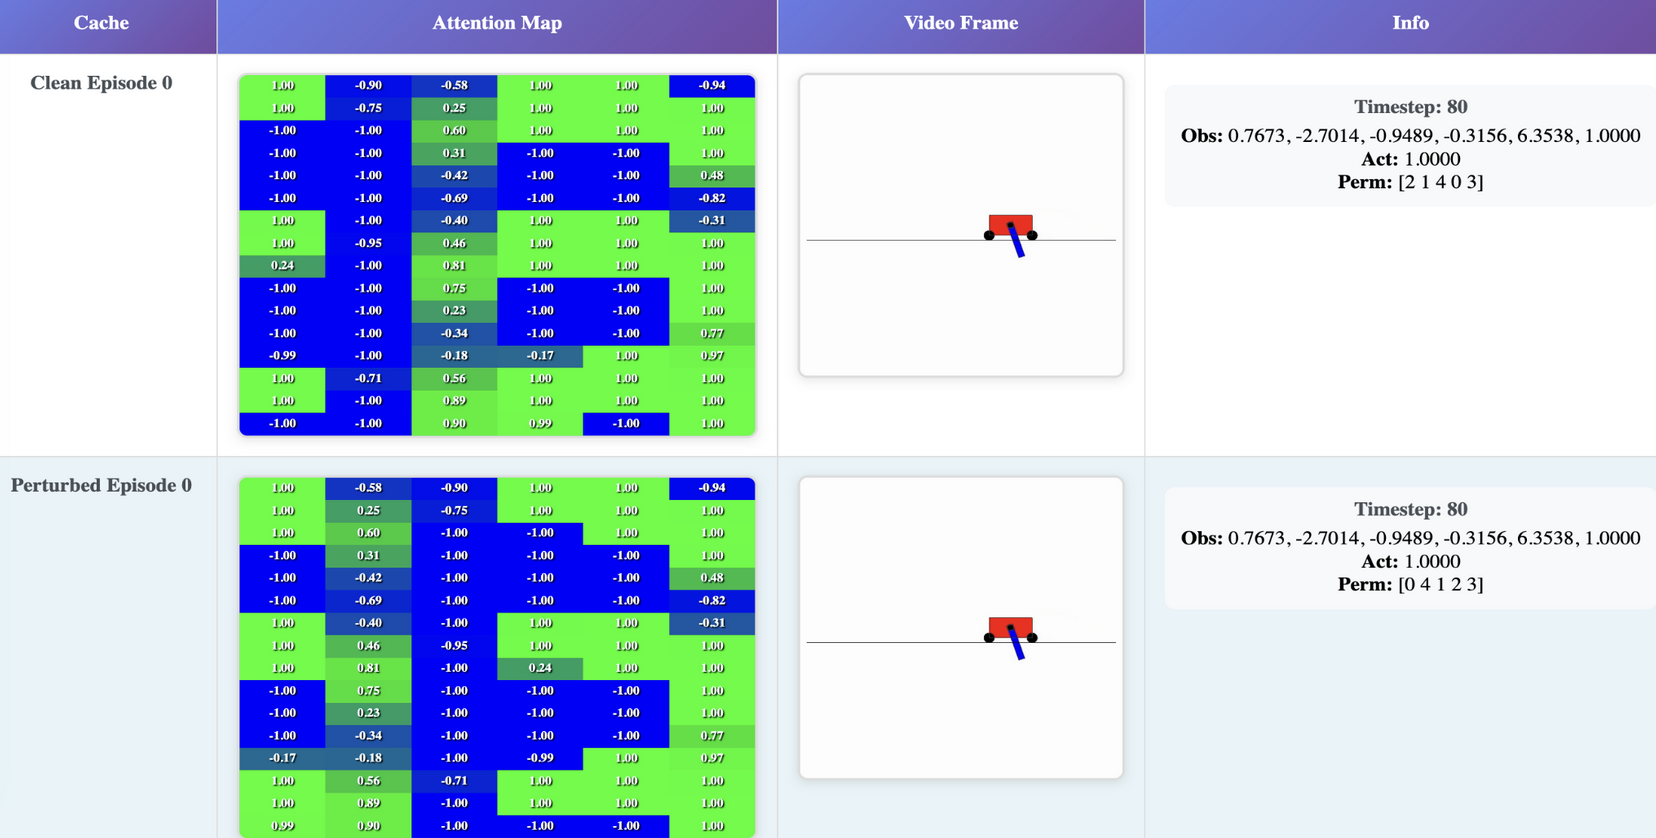
\includegraphics[width=\textwidth]{images/is_perm_iv.png}
    \caption{When the LSTM recurrent state is zeroed at every time step, the columns in the attention matrix have been permuted in the same way as the observation vector's rows. 
    In this specific circumstance, we do see that the Attention Neuron architecture is permutation invariant.}
    \label{fig:attention_neuron_permutation_invariance_zeroed_lstm}
\end{figure}

This finding has some startling implications.
For one, it shows that the Attention Neuron architecture
can achieve robustness to permutation observations within episodes,
even when its LSTM recurrent states have made the policy permutation sensitive overall.

This suggests that the architecture could have learned to rely on certain features of the input
that are invariant to permutations, allowing it to maintain performance despite changes
in the order of the input sequence.

\section{Future Work}

% New Scenarios!
% Ant, CarRacing, Pong
% Examine Noisy Channels
% Another feature in paper
% Conduct More Ablations
% Hidden Layers, Attention (Ablate by column and output feature (row).)
% Optimize Model Performance
% Authors used evolutionary strategy; invested very little compute per model trained.
% 4096 episodes ~= 250K-1M timesteps 
% Possible we don't see meaningful features as a result
% Analyze Train-Time Evolution
% When do the features emerge?

In future work, we would like to explore the following directions:
\begin{itemize}
    \item \textbf{Testing on More Complex Environments}:
        We have thus far been focused on the mechanistic and architectural properties of the Attention Neuron.
        However, it would be interesting to see how the Attention Neuron architecture performs
        on more complex environments such as Ant, CarRacing, and Pong.
    \item \textbf{Examining Noisy Channels}:
        The authors \cite{Tang-and-Ha-2021} also state that the Attention Neuron architecture
        is robust to extraneous, noisy channels in the observation vector.
        A natural extension to our study is to analyze why this is the case, and whether the architecture
        can be made more robust to noisy channels.
    \item \textbf{Conducting More Ablations}:
        We have only conducted a few ablations on the Attention Neuron architecture.
        It would be interesting to conduct more ablations, such as ablations on the attention matrix,
        position embeddings, and information signals.
    \item \textbf{Optimizing Model Performance}:
        The authors \cite{Tang-and-Ha-2021} used an evolutionary strategy to 
        optimize the performance of the Attention Neuron architecture \textit{given a fixed compute budget},
        by searching over multiple training instances simultaneously.
        However, this could mean that any individual model's potential is not fully realized,
        especially for more complex environments.
        Learning about the features which emerge over the course of training
        could also help us understand how the Attention Neuron architecture learns to be robust to permutations.

\end{itemize}

\bibliographystyle{unsrt}
\bibliography{main.bib}
\end{document}
